
%(BEGIN_QUESTION)
% Copyright 2009, Tony R. Kuphaldt, released under the Creative Commons Attribution License (v 1.0)
% This means you may do almost anything with this work of mine, so long as you give me proper credit

Some models of the ``MicroLogix'' series of programmable logic controller (PLC) manufactured by Allen-Bradley come equipped with analog inputs, designed to receive either voltage or current signals from analog sensors.  Examine the internal resistances of the analog inputs (IA/0, IA/1, IA/2, and IA/3) to determine which are designed to input voltage signals and which are designed to input current signals.

$$\includegraphics[width=15.5cm]{i03811x01.eps}$$

Hint: think in terms of the input resistances of {\it voltmeters} and {\it ammeters}.  Which of these test instrument types are known for having very large input resistance values?   Which of these test instrument types are known for having very small input resistance values?

\vskip 10pt

Assuming the three sensors shown all have internal power sources (no need for an external DC power supply to make them output their respective signals), draw connecting wires between these sensors and the appropriate inputs on the PLC.

\underbar{file i03811}
%(END_QUESTION)





%(BEGIN_ANSWER)

IA/0 and IA/1 are both analog {\it voltage} inputs.  We know this because of their large input resistances (210 k$\Omega$).

\vskip 10pt

IA/2 and IA/3 are both analog {\it current} inputs.  We know this because of their small input resistances (160 $\Omega$).

\vskip 10pt

$$\includegraphics[width=15.5cm]{i03811x02.eps}$$

%(END_ANSWER)





%(BEGIN_NOTES)

%INDEX% Pictorial circuit review (distinguishing voltage versus current analog inputs)

%(END_NOTES)


